\documentclass[1p]{elsarticle_modified}
%\bibliographystyle{elsarticle-num}

%\usepackage[colorlinks]{hyperref}
%\usepackage{abbrmath_seonhwa} %\Abb, \Ascr, \Acal ,\Abf, \Afrak
\usepackage{amsfonts}
\usepackage{amssymb}
\usepackage{amsmath}
\usepackage{amsthm}
\usepackage{scalefnt}
\usepackage{amsbsy}
\usepackage{kotex}
\usepackage{caption}
\usepackage{subfig}
\usepackage{color}
\usepackage{graphicx}
\usepackage{xcolor} %% white, black, red, green, blue, cyan, magenta, yellow
\usepackage{float}
\usepackage{setspace}
\usepackage{hyperref}

\usepackage{tikz}
\usetikzlibrary{arrows}

\usepackage{multirow}
\usepackage{array} % fixed length table
\usepackage{hhline}

%%%%%%%%%%%%%%%%%%%%%
\makeatletter
\renewcommand*\env@matrix[1][\arraystretch]{%
	\edef\arraystretch{#1}%
	\hskip -\arraycolsep
	\let\@ifnextchar\new@ifnextchar
	\array{*\c@MaxMatrixCols c}}
\makeatother %https://tex.stackexchange.com/questions/14071/how-can-i-increase-the-line-spacing-in-a-matrix
%%%%%%%%%%%%%%%

\usepackage[normalem]{ulem}

\newcommand{\msout}[1]{\ifmmode\text{\sout{\ensuremath{#1}}}\else\sout{#1}\fi}
%SOURCE: \msout is \stkout macro in https://tex.stackexchange.com/questions/20609/strikeout-in-math-mode

\newcommand{\cancel}[1]{
	\ifmmode
	{\color{red}\msout{#1}}
	\else
	{\color{red}\sout{#1}}
	\fi
}

\newcommand{\add}[1]{
	{\color{blue}\uwave{#1}}
}

\newcommand{\replace}[2]{
	\ifmmode
	{\color{red}\msout{#1}}{\color{blue}\uwave{#2}}
	\else
	{\color{red}\sout{#1}}{\color{blue}\uwave{#2}}
	\fi
}

\newcommand{\Sol}{\mathcal{S}} %segment
\newcommand{\D}{D} %diagram
\newcommand{\A}{\mathcal{A}} %arc


%%%%%%%%%%%%%%%%%%%%%%%%%%%%%5 test

\def\sl{\operatorname{\textup{SL}}(2,\Cbb)}
\def\psl{\operatorname{\textup{PSL}}(2,\Cbb)}
\def\quan{\mkern 1mu \triangleright \mkern 1mu}

\theoremstyle{definition}
\newtheorem{thm}{Theorem}[section]
\newtheorem{prop}[thm]{Proposition}
\newtheorem{lem}[thm]{Lemma}
\newtheorem{ques}[thm]{Question}
\newtheorem{cor}[thm]{Corollary}
\newtheorem{defn}[thm]{Definition}
\newtheorem{exam}[thm]{Example}
\newtheorem{rmk}[thm]{Remark}
\newtheorem{alg}[thm]{Algorithm}

\newcommand{\I}{\sqrt{-1}}
\begin{document}

%\begin{frontmatter}
%
%\title{Boundary parabolic representations of knots up to 8 crossings}
%
%%% Group authors per affiliation:
%\author{Yunhi Cho} 
%\address{Department of Mathematics, University of Seoul, Seoul, Korea}
%\ead{yhcho@uos.ac.kr}
%
%
%\author{Seonhwa Kim} %\fnref{s_kim}}
%\address{Center for Geometry and Physics, Institute for Basic Science, Pohang, 37673, Korea}
%\ead{ryeona17@ibs.re.kr}
%
%\author{Hyuk Kim}
%\address{Department of Mathematical Sciences, Seoul National University, Seoul 08826, Korea}
%\ead{hyukkim@snu.ac.kr}
%
%\author{Seokbeom Yoon}
%\address{Department of Mathematical Sciences, Seoul National University, Seoul, 08826,  Korea}
%\ead{sbyoon15@snu.ac.kr}
%
%\begin{abstract}
%We find all boundary parabolic representation of knots up to 8 crossings.
%
%\end{abstract}
%\begin{keyword}
%    \MSC[2010] 57M25 
%\end{keyword}
%
%\end{frontmatter}

%\linenumbers
%\tableofcontents
%
\newcommand\colored[1]{\textcolor{white}{\rule[-0.35ex]{0.8em}{1.4ex}}\kern-0.8em\color{red} #1}%
%\newcommand\colored[1]{\textcolor{white}{ #1}\kern-2.17ex	\textcolor{white}{ #1}\kern-1.81ex	\textcolor{white}{ #1}\kern-2.15ex\color{red}#1	}

{\Large $\underline{12n_{0167}~(K12n_{0167})}$}

\setlength{\tabcolsep}{10pt}
\renewcommand{\arraystretch}{1.6}
\vspace{1cm}\begin{tabular}{m{100pt}>{\centering\arraybackslash}m{274pt}}
\multirow{5}{120pt}{
	\centering
	\includegraphics[width=112pt]{../../../GIT/diagram.site/Diagrams/png/2256_12n_0167.png}\\
\ \ \ A knot diagram\footnotemark}&
\allowdisplaybreaks
\textbf{Linearized knot diagam} \\
\cline{2-2}
 &
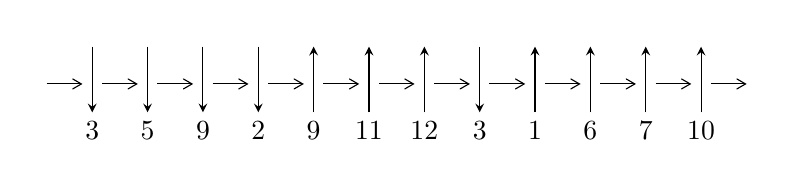
\begin{tikzpicture}[x=20pt, y=17pt]
	% nodes
	\node (C0) at (0, 0) {};
	\node (C1) at (1, 0) {};
	\node (C1U) at (1, +1) {};
	\node (C1D) at (1, -1) {3};

	\node (C2) at (2, 0) {};
	\node (C2U) at (2, +1) {};
	\node (C2D) at (2, -1) {5};

	\node (C3) at (3, 0) {};
	\node (C3U) at (3, +1) {};
	\node (C3D) at (3, -1) {9};

	\node (C4) at (4, 0) {};
	\node (C4U) at (4, +1) {};
	\node (C4D) at (4, -1) {2};

	\node (C5) at (5, 0) {};
	\node (C5U) at (5, +1) {};
	\node (C5D) at (5, -1) {9};

	\node (C6) at (6, 0) {};
	\node (C6U) at (6, +1) {};
	\node (C6D) at (6, -1) {11};

	\node (C7) at (7, 0) {};
	\node (C7U) at (7, +1) {};
	\node (C7D) at (7, -1) {12};

	\node (C8) at (8, 0) {};
	\node (C8U) at (8, +1) {};
	\node (C8D) at (8, -1) {3};

	\node (C9) at (9, 0) {};
	\node (C9U) at (9, +1) {};
	\node (C9D) at (9, -1) {1};

	\node (C10) at (10, 0) {};
	\node (C10U) at (10, +1) {};
	\node (C10D) at (10, -1) {6};

	\node (C11) at (11, 0) {};
	\node (C11U) at (11, +1) {};
	\node (C11D) at (11, -1) {7};

	\node (C12) at (12, 0) {};
	\node (C12U) at (12, +1) {};
	\node (C12D) at (12, -1) {10};
	\node (C13) at (13, 0) {};

	% arrows
	\draw[->,>={angle 60}]
	(C0) edge (C1) (C1) edge (C2) (C2) edge (C3) (C3) edge (C4) (C4) edge (C5) (C5) edge (C6) (C6) edge (C7) (C7) edge (C8) (C8) edge (C9) (C9) edge (C10) (C10) edge (C11) (C11) edge (C12) (C12) edge (C13) ;	\draw[->,>=stealth]
	(C1U) edge (C1D) (C2U) edge (C2D) (C3U) edge (C3D) (C4U) edge (C4D) (C5D) edge (C5U) (C6D) edge (C6U) (C7D) edge (C7U) (C8U) edge (C8D) (C9D) edge (C9U) (C10D) edge (C10U) (C11D) edge (C11U) (C12D) edge (C12U) ;
	\end{tikzpicture} \\
\hhline{~~} \\& 
\textbf{Solving Sequence} \\ \cline{2-2} 
 &
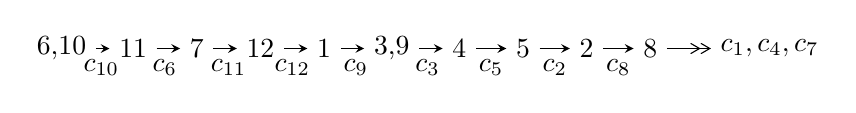
\begin{tikzpicture}[x=23pt, y=7pt]
	% node
	\node (A0) at (-1/8, 0) {6,10};
	\node (A1) at (1, 0) {11};
	\node (A2) at (2, 0) {7};
	\node (A3) at (3, 0) {12};
	\node (A4) at (4, 0) {1};
	\node (A5) at (81/16, 0) {3,9};
	\node (A6) at (49/8, 0) {4};
	\node (A7) at (57/8, 0) {5};
	\node (A8) at (65/8, 0) {2};
	\node (A9) at (73/8, 0) {8};
	\node (C1) at (1/2, -1) {$c_{10}$};
	\node (C2) at (3/2, -1) {$c_{6}$};
	\node (C3) at (5/2, -1) {$c_{11}$};
	\node (C4) at (7/2, -1) {$c_{12}$};
	\node (C5) at (9/2, -1) {$c_{9}$};
	\node (C6) at (45/8, -1) {$c_{3}$};
	\node (C7) at (53/8, -1) {$c_{5}$};
	\node (C8) at (61/8, -1) {$c_{2}$};
	\node (C9) at (69/8, -1) {$c_{8}$};
	\node (A10) at (11, 0) {$c_{1},c_{4},c_{7}$};

	% edge
	\draw[->,>=stealth]	
	(A0) edge (A1) (A1) edge (A2) (A2) edge (A3) (A3) edge (A4) (A4) edge (A5) (A5) edge (A6) (A6) edge (A7) (A7) edge (A8) (A8) edge (A9) ;
	\draw[->>,>={angle 60}]	
	(A9) edge (A10);
\end{tikzpicture} \\ 

\end{tabular} \\

\footnotetext{
The image of knot diagram is generated by the software ``\textbf{Draw programme}" developed by Andrew Bartholomew(\url{http://www.layer8.co.uk/maths/draw/index.htm\#Running-draw}), where we modified some parts for our purpose(\url{https://github.com/CATsTAILs/LinksPainter}).
}\phantom \\ \newline 
\centering \textbf{Ideals for irreducible components\footnotemark of $X_{\text{par}}$} 
 
\begin{align*}
I^u_{1}&=\langle 
2 u^{38}-42 u^{36}+\cdots+b+2,\;- u^{38}- u^{37}+\cdots+a-2,\;u^{39}+2 u^{38}+\cdots+2 u+1\rangle \\
I^u_{2}&=\langle 
u^4-2 u^2+b,\;- u^5+u^4+3 u^3-2 u^2+a-2 u-1,\;u^6- u^5-3 u^4+2 u^3+2 u^2+u-1\rangle \\
\\
\end{align*}
\raggedright * 2 irreducible components of $\dim_{\mathbb{C}}=0$, with total 45 representations.\\
\footnotetext{All coefficients of polynomials are rational numbers. But the coefficients are sometimes approximated in decimal forms when there is not enough margin.}
\newpage
\renewcommand{\arraystretch}{1}
\centering \section*{I. $I^u_{1}= \langle 2 u^{38}-42 u^{36}+\cdots+b+2,\;- u^{38}- u^{37}+\cdots+a-2,\;u^{39}+2 u^{38}+\cdots+2 u+1 \rangle$}
\flushleft \textbf{(i) Arc colorings}\\
\begin{tabular}{m{7pt} m{180pt} m{7pt} m{180pt} }
\flushright $a_{6}=$&$\begin{pmatrix}0\\u\end{pmatrix}$ \\
\flushright $a_{10}=$&$\begin{pmatrix}1\\0\end{pmatrix}$ \\
\flushright $a_{11}=$&$\begin{pmatrix}1\\- u^2\end{pmatrix}$ \\
\flushright $a_{7}=$&$\begin{pmatrix}u\\- u^3+u\end{pmatrix}$ \\
\flushright $a_{12}=$&$\begin{pmatrix}- u^2+1\\u^4-2 u^2\end{pmatrix}$ \\
\flushright $a_{1}=$&$\begin{pmatrix}u^4-3 u^2+1\\u^4-2 u^2\end{pmatrix}$ \\
\flushright $a_{3}=$&$\begin{pmatrix}u^{38}+u^{37}+\cdots-7 u+2\\-2 u^{38}+42 u^{36}+\cdots-5 u-2\end{pmatrix}$ \\
\flushright $a_{9}=$&$\begin{pmatrix}u^8-5 u^6+7 u^4-2 u^2+1\\u^8-4 u^6+4 u^4\end{pmatrix}$ \\
\flushright $a_{4}=$&$\begin{pmatrix}u^{38}+u^{37}+\cdots-8 u+1\\-4 u^{38}+84 u^{36}+\cdots-8 u-4\end{pmatrix}$ \\
\flushright $a_{5}=$&$\begin{pmatrix}- u^{17}+10 u^{15}-39 u^{13}+74 u^{11}-71 u^9+38 u^7-18 u^5+4 u^3- u\\- u^{17}+9 u^{15}-31 u^{13}+50 u^{11}-37 u^9+12 u^7-4 u^5+u\end{pmatrix}$ \\
\flushright $a_{2}=$&$\begin{pmatrix}u^{38}+u^{37}+\cdots-5 u+3\\- u^{38}+21 u^{36}+\cdots-3 u-1\end{pmatrix}$ \\
\flushright $a_{8}=$&$\begin{pmatrix}- u^3+2 u\\u^5-3 u^3+u\end{pmatrix}$\\&\end{tabular}
\flushleft \textbf{(ii) Obstruction class $= -1$}\\~\\
\flushleft \textbf{(iii) Cusp Shapes $= -8 u^{38}-11 u^{37}+\cdots+34 u-6$}\\~\\
\newpage\renewcommand{\arraystretch}{1}
\flushleft \textbf{(iv) u-Polynomials at the component}\newline \\
\begin{tabular}{m{50pt}|m{274pt}}
Crossings & \hspace{64pt}u-Polynomials at each crossing \\
\hline $$\begin{aligned}c_{1}\end{aligned}$$&$\begin{aligned}
&u^{39}+11 u^{38}+\cdots-5 u+1
\end{aligned}$\\
\hline $$\begin{aligned}c_{2},c_{4}\end{aligned}$$&$\begin{aligned}
&u^{39}-7 u^{38}+\cdots-3 u+1
\end{aligned}$\\
\hline $$\begin{aligned}c_{3},c_{8}\end{aligned}$$&$\begin{aligned}
&u^{39}+u^{38}+\cdots+64 u+64
\end{aligned}$\\
\hline $$\begin{aligned}c_{5}\end{aligned}$$&$\begin{aligned}
&u^{39}-2 u^{38}+\cdots+2 u+1
\end{aligned}$\\
\hline $$\begin{aligned}c_{6},c_{7},c_{10}\\c_{11}\end{aligned}$$&$\begin{aligned}
&u^{39}+2 u^{38}+\cdots+2 u+1
\end{aligned}$\\
\hline $$\begin{aligned}c_{9},c_{12}\end{aligned}$$&$\begin{aligned}
&u^{39}+8 u^{38}+\cdots+70 u-7
\end{aligned}$\\
\hline
\end{tabular}\\~\\
\newpage\renewcommand{\arraystretch}{1}
\flushleft \textbf{(v) Riley Polynomials at the component}\newline \\
\begin{tabular}{m{50pt}|m{274pt}}
Crossings & \hspace{64pt}Riley Polynomials at each crossing \\
\hline $$\begin{aligned}c_{1}\end{aligned}$$&$\begin{aligned}
&y^{39}+41 y^{38}+\cdots+87 y-1
\end{aligned}$\\
\hline $$\begin{aligned}c_{2},c_{4}\end{aligned}$$&$\begin{aligned}
&y^{39}-11 y^{38}+\cdots-5 y-1
\end{aligned}$\\
\hline $$\begin{aligned}c_{3},c_{8}\end{aligned}$$&$\begin{aligned}
&y^{39}+39 y^{38}+\cdots-24576 y-4096
\end{aligned}$\\
\hline $$\begin{aligned}c_{5}\end{aligned}$$&$\begin{aligned}
&y^{39}-44 y^{38}+\cdots+26 y-1
\end{aligned}$\\
\hline $$\begin{aligned}c_{6},c_{7},c_{10}\\c_{11}\end{aligned}$$&$\begin{aligned}
&y^{39}-44 y^{38}+\cdots+26 y-1
\end{aligned}$\\
\hline $$\begin{aligned}c_{9},c_{12}\end{aligned}$$&$\begin{aligned}
&y^{39}+16 y^{38}+\cdots+3318 y-49
\end{aligned}$\\
\hline
\end{tabular}\\~\\
\newpage\flushleft \textbf{(vi) Complex Volumes and Cusp Shapes}
$$\begin{array}{c|c|c}  
\text{Solutions to }I^u_{1}& \I (\text{vol} + \sqrt{-1}CS) & \text{Cusp shape}\\
 \hline 
\begin{aligned}
u &= -0.929287 + 0.081478 I \\
a &= -0.13426 + 1.82517 I \\
b &= -0.120150 + 0.122224 I\end{aligned}
 & \phantom{-}7.67542 - 3.35786 I & \phantom{-}7.74116 + 3.09384 I \\ \hline\begin{aligned}
u &= -0.929287 - 0.081478 I \\
a &= -0.13426 - 1.82517 I \\
b &= -0.120150 - 0.122224 I\end{aligned}
 & \phantom{-}7.67542 + 3.35786 I & \phantom{-}7.74116 - 3.09384 I \\ \hline\begin{aligned}
u &= \phantom{-}0.638465 + 0.572171 I \\
a &= \phantom{-}0.99563 + 1.99588 I \\
b &= \phantom{-}2.30175 + 0.94966 I\end{aligned}
 & \phantom{-}3.77609 + 9.59779 I & \phantom{-}3.17812 - 7.93232 I \\ \hline\begin{aligned}
u &= \phantom{-}0.638465 - 0.572171 I \\
a &= \phantom{-}0.99563 - 1.99588 I \\
b &= \phantom{-}2.30175 - 0.94966 I\end{aligned}
 & \phantom{-}3.77609 - 9.59779 I & \phantom{-}3.17812 + 7.93232 I \\ \hline\begin{aligned}
u &= \phantom{-}0.662133 + 0.524823 I \\
a &= -0.67104 - 1.69728 I \\
b &= -1.95714 - 0.96279 I\end{aligned}
 & \phantom{-}4.90817 + 2.86742 I & \phantom{-}5.04494 - 3.58436 I \\ \hline\begin{aligned}
u &= \phantom{-}0.662133 - 0.524823 I \\
a &= -0.67104 + 1.69728 I \\
b &= -1.95714 + 0.96279 I\end{aligned}
 & \phantom{-}4.90817 - 2.86742 I & \phantom{-}5.04494 + 3.58436 I \\ \hline\begin{aligned}
u &= -0.494019 + 0.600246 I \\
a &= \phantom{-}0.252653 + 0.393043 I \\
b &= \phantom{-}0.096843 + 0.148262 I\end{aligned}
 & -3.75312 - 2.04581 I & \phantom{-}4.95801 + 3.83439 I \\ \hline\begin{aligned}
u &= -0.494019 - 0.600246 I \\
a &= \phantom{-}0.252653 - 0.393043 I \\
b &= \phantom{-}0.096843 - 0.148262 I\end{aligned}
 & -3.75312 + 2.04581 I & \phantom{-}4.95801 - 3.83439 I \\ \hline\begin{aligned}
u &= -0.567091 + 0.480850 I \\
a &= -0.585871 + 0.875832 I \\
b &= -0.215752 + 0.266566 I\end{aligned}
 & -1.26346 - 3.63942 I & \phantom{-}1.82295 + 7.50238 I \\ \hline\begin{aligned}
u &= -0.567091 - 0.480850 I \\
a &= -0.585871 - 0.875832 I \\
b &= -0.215752 - 0.266566 I\end{aligned}
 & -1.26346 + 3.63942 I & \phantom{-}1.82295 - 7.50238 I\\
 \hline 
 \end{array}$$\newpage$$\begin{array}{c|c|c}  
\text{Solutions to }I^u_{1}& \I (\text{vol} + \sqrt{-1}CS) & \text{Cusp shape}\\
 \hline 
\begin{aligned}
u &= \phantom{-}0.307625 + 0.630440 I \\
a &= -2.49493 - 0.52608 I \\
b &= -1.53447 + 0.98532 I\end{aligned}
 & \phantom{-}2.80401 - 5.51652 I & \phantom{-}1.04879 + 2.33706 I \\ \hline\begin{aligned}
u &= \phantom{-}0.307625 - 0.630440 I \\
a &= -2.49493 + 0.52608 I \\
b &= -1.53447 - 0.98532 I\end{aligned}
 & \phantom{-}2.80401 + 5.51652 I & \phantom{-}1.04879 - 2.33706 I \\ \hline\begin{aligned}
u &= \phantom{-}0.487298 + 0.473095 I \\
a &= -1.50995 + 1.72805 I \\
b &= \phantom{-}0.60093 + 2.21671 I\end{aligned}
 & -3.11331 + 1.66779 I & \phantom{-}1.80697 - 3.74196 I \\ \hline\begin{aligned}
u &= \phantom{-}0.487298 - 0.473095 I \\
a &= -1.50995 - 1.72805 I \\
b &= \phantom{-}0.60093 - 2.21671 I\end{aligned}
 & -3.11331 - 1.66779 I & \phantom{-}1.80697 + 3.74196 I \\ \hline\begin{aligned}
u &= \phantom{-}0.237194 + 0.597912 I \\
a &= \phantom{-}2.21111 + 0.47598 I \\
b &= \phantom{-}1.19865 - 0.81016 I\end{aligned}
 & \phantom{-}3.66747 + 0.95204 I & \phantom{-}2.02608 - 2.37857 I \\ \hline\begin{aligned}
u &= \phantom{-}0.237194 - 0.597912 I \\
a &= \phantom{-}2.21111 - 0.47598 I \\
b &= \phantom{-}1.19865 + 0.81016 I\end{aligned}
 & \phantom{-}3.66747 - 0.95204 I & \phantom{-}2.02608 + 2.37857 I \\ \hline\begin{aligned}
u &= -1.373730 + 0.070434 I \\
a &= \phantom{-}0.257891 - 1.073270 I \\
b &= \phantom{-}0.278657 + 1.104960 I\end{aligned}
 & \phantom{-}7.90973 + 2.98789 I & \phantom{-0.000000 } 0 \\ \hline\begin{aligned}
u &= -1.373730 - 0.070434 I \\
a &= \phantom{-}0.257891 + 1.073270 I \\
b &= \phantom{-}0.278657 - 1.104960 I\end{aligned}
 & \phantom{-}7.90973 - 2.98789 I & \phantom{-0.000000 } 0 \\ \hline\begin{aligned}
u &= -0.376548 + 0.452986 I \\
a &= \phantom{-}1.297760 - 0.214121 I \\
b &= \phantom{-}0.390433 - 0.135895 I\end{aligned}
 & -1.82437 + 0.31015 I & -1.43952 + 0.71227 I \\ \hline\begin{aligned}
u &= -0.376548 - 0.452986 I \\
a &= \phantom{-}1.297760 + 0.214121 I \\
b &= \phantom{-}0.390433 + 0.135895 I\end{aligned}
 & -1.82437 - 0.31015 I & -1.43952 - 0.71227 I\\
 \hline 
 \end{array}$$\newpage$$\begin{array}{c|c|c}  
\text{Solutions to }I^u_{1}& \I (\text{vol} + \sqrt{-1}CS) & \text{Cusp shape}\\
 \hline 
\begin{aligned}
u &= \phantom{-}0.570048 + 0.105370 I \\
a &= \phantom{-}0.117467 - 0.126119 I \\
b &= -0.536626 - 0.310271 I\end{aligned}
 & \phantom{-}0.990011 + 0.147928 I & \phantom{-}10.02163 - 0.80608 I \\ \hline\begin{aligned}
u &= \phantom{-}0.570048 - 0.105370 I \\
a &= \phantom{-}0.117467 + 0.126119 I \\
b &= -0.536626 + 0.310271 I\end{aligned}
 & \phantom{-}0.990011 - 0.147928 I & \phantom{-}10.02163 + 0.80608 I \\ \hline\begin{aligned}
u &= \phantom{-}1.51500 + 0.17385 I \\
a &= -0.236905 + 0.112592 I \\
b &= -0.307436 + 0.170867 I\end{aligned}
 & \phantom{-}2.85829 + 4.80629 I & \phantom{-0.000000 } 0 \\ \hline\begin{aligned}
u &= \phantom{-}1.51500 - 0.17385 I \\
a &= -0.236905 - 0.112592 I \\
b &= -0.307436 - 0.170867 I\end{aligned}
 & \phantom{-}2.85829 - 4.80629 I & \phantom{-0.000000 } 0 \\ \hline\begin{aligned}
u &= \phantom{-}1.52238 + 0.09213 I \\
a &= -0.528996 - 0.528049 I \\
b &= -0.736761 - 0.687194 I\end{aligned}
 & \phantom{-}4.57565 + 1.35883 I & \phantom{-0.000000 } 0 \\ \hline\begin{aligned}
u &= \phantom{-}1.52238 - 0.09213 I \\
a &= -0.528996 + 0.528049 I \\
b &= -0.736761 + 0.687194 I\end{aligned}
 & \phantom{-}4.57565 - 1.35883 I & \phantom{-0.000000 } 0 \\ \hline\begin{aligned}
u &= -1.53584 + 0.12162 I \\
a &= \phantom{-}1.040540 + 0.300970 I \\
b &= -1.70605 + 2.33955 I\end{aligned}
 & \phantom{-}3.67223 - 3.72431 I & \phantom{-0.000000 } 0 \\ \hline\begin{aligned}
u &= -1.53584 - 0.12162 I \\
a &= \phantom{-}1.040540 - 0.300970 I \\
b &= -1.70605 - 2.33955 I\end{aligned}
 & \phantom{-}3.67223 + 3.72431 I & \phantom{-0.000000 } 0 \\ \hline\begin{aligned}
u &= -1.55793 + 0.04362 I \\
a &= -0.237922 - 0.022146 I \\
b &= \phantom{-}1.048690 - 0.750159 I\end{aligned}
 & \phantom{-}8.23625 - 0.76574 I & \phantom{-0.000000 } 0 \\ \hline\begin{aligned}
u &= -1.55793 - 0.04362 I \\
a &= -0.237922 + 0.022146 I \\
b &= \phantom{-}1.048690 + 0.750159 I\end{aligned}
 & \phantom{-}8.23625 + 0.76574 I & \phantom{-0.000000 } 0\\
 \hline 
 \end{array}$$\newpage$$\begin{array}{c|c|c}  
\text{Solutions to }I^u_{1}& \I (\text{vol} + \sqrt{-1}CS) & \text{Cusp shape}\\
 \hline 
\begin{aligned}
u &= \phantom{-}1.55813 + 0.13570 I \\
a &= \phantom{-}0.109432 + 0.550566 I \\
b &= \phantom{-}0.178775 + 0.723045 I\end{aligned}
 & \phantom{-}5.88421 + 5.85782 I & \phantom{-0.000000 } 0 \\ \hline\begin{aligned}
u &= \phantom{-}1.55813 - 0.13570 I \\
a &= \phantom{-}0.109432 - 0.550566 I \\
b &= \phantom{-}0.178775 - 0.723045 I\end{aligned}
 & \phantom{-}5.88421 - 5.85782 I & \phantom{-0.000000 } 0 \\ \hline\begin{aligned}
u &= -1.57931 + 0.17338 I \\
a &= \phantom{-}0.210755 + 1.250430 I \\
b &= -2.99968 + 0.82586 I\end{aligned}
 & \phantom{-}11.2088 - 12.3506 I & \phantom{-0.000000 } 0 \\ \hline\begin{aligned}
u &= -1.57931 - 0.17338 I \\
a &= \phantom{-}0.210755 - 1.250430 I \\
b &= -2.99968 - 0.82586 I\end{aligned}
 & \phantom{-}11.2088 + 12.3506 I & \phantom{-0.000000 } 0 \\ \hline\begin{aligned}
u &= -1.58740 + 0.15498 I \\
a &= -0.271413 - 1.006140 I \\
b &= \phantom{-}2.71217 - 1.00066 I\end{aligned}
 & \phantom{-}12.48550 - 5.38089 I & \phantom{-0.000000 } 0 \\ \hline\begin{aligned}
u &= -1.58740 - 0.15498 I \\
a &= -0.271413 + 1.006140 I \\
b &= \phantom{-}2.71217 + 1.00066 I\end{aligned}
 & \phantom{-}12.48550 + 5.38089 I & \phantom{-0.000000 } 0 \\ \hline\begin{aligned}
u &= \phantom{-}1.62512 + 0.01288 I \\
a &= \phantom{-}0.034213 + 1.205770 I \\
b &= \phantom{-}0.05087 + 1.57468 I\end{aligned}
 & \phantom{-}16.3023 + 3.6362 I & \phantom{-0.000000 } 0 \\ \hline\begin{aligned}
u &= \phantom{-}1.62512 - 0.01288 I \\
a &= \phantom{-}0.034213 - 1.205770 I \\
b &= \phantom{-}0.05087 - 1.57468 I\end{aligned}
 & \phantom{-}16.3023 - 3.6362 I & \phantom{-0.000000 } 0 \\ \hline\begin{aligned}
u &= -0.244498\phantom{ +0.000000I} \\
a &= \phantom{-}3.28769\phantom{ +0.000000I} \\
b &= \phantom{-}0.512609\phantom{ +0.000000I}\end{aligned}
 & -1.28163\phantom{ +0.000000I} & -11.2860\phantom{ +0.000000I}\\
 \hline 
 \end{array}$$\newpage\newpage\renewcommand{\arraystretch}{1}
\centering \section*{II. $I^u_{2}= \langle u^4-2 u^2+b,\;- u^5+u^4+3 u^3-2 u^2+a-2 u-1,\;u^6- u^5-3 u^4+2 u^3+2 u^2+u-1 \rangle$}
\flushleft \textbf{(i) Arc colorings}\\
\begin{tabular}{m{7pt} m{180pt} m{7pt} m{180pt} }
\flushright $a_{6}=$&$\begin{pmatrix}0\\u\end{pmatrix}$ \\
\flushright $a_{10}=$&$\begin{pmatrix}1\\0\end{pmatrix}$ \\
\flushright $a_{11}=$&$\begin{pmatrix}1\\- u^2\end{pmatrix}$ \\
\flushright $a_{7}=$&$\begin{pmatrix}u\\- u^3+u\end{pmatrix}$ \\
\flushright $a_{12}=$&$\begin{pmatrix}- u^2+1\\u^4-2 u^2\end{pmatrix}$ \\
\flushright $a_{1}=$&$\begin{pmatrix}u^4-3 u^2+1\\u^4-2 u^2\end{pmatrix}$ \\
\flushright $a_{3}=$&$\begin{pmatrix}u^5- u^4-3 u^3+2 u^2+2 u+1\\- u^4+2 u^2\end{pmatrix}$ \\
\flushright $a_{9}=$&$\begin{pmatrix}- u^3+2 u\\u^5-3 u^3+u\end{pmatrix}$ \\
\flushright $a_{4}=$&$\begin{pmatrix}u^5- u^4-3 u^3+2 u^2+2 u+1\\- u^4+2 u^2\end{pmatrix}$ \\
\flushright $a_{5}=$&$\begin{pmatrix}- u^4+3 u^2-1\\- u^4+2 u^2\end{pmatrix}$ \\
\flushright $a_{2}=$&$\begin{pmatrix}u^5-3 u^3- u^2+2 u+2\\0\end{pmatrix}$ \\
\flushright $a_{8}=$&$\begin{pmatrix}- u^3+2 u\\u^5-3 u^3+u\end{pmatrix}$\\&\end{tabular}
\flushleft \textbf{(ii) Obstruction class $= 1$}\\~\\
\flushleft \textbf{(iii) Cusp Shapes $= 3 u^5- u^4-14 u^3+u^2+14 u+6$}\\~\\
\newpage\renewcommand{\arraystretch}{1}
\flushleft \textbf{(iv) u-Polynomials at the component}\newline \\
\begin{tabular}{m{50pt}|m{274pt}}
Crossings & \hspace{64pt}u-Polynomials at each crossing \\
\hline $$\begin{aligned}c_{1},c_{2}\end{aligned}$$&$\begin{aligned}
&(u-1)^6
\end{aligned}$\\
\hline $$\begin{aligned}c_{3},c_{8}\end{aligned}$$&$\begin{aligned}
&u^6
\end{aligned}$\\
\hline $$\begin{aligned}c_{4}\end{aligned}$$&$\begin{aligned}
&(u+1)^6
\end{aligned}$\\
\hline $$\begin{aligned}c_{5},c_{9}\end{aligned}$$&$\begin{aligned}
&u^6- u^5+3 u^4-2 u^3+2 u^2- u-1
\end{aligned}$\\
\hline $$\begin{aligned}c_{6},c_{7}\end{aligned}$$&$\begin{aligned}
&u^6+u^5-3 u^4-2 u^3+2 u^2- u-1
\end{aligned}$\\
\hline $$\begin{aligned}c_{10},c_{11}\end{aligned}$$&$\begin{aligned}
&u^6- u^5-3 u^4+2 u^3+2 u^2+u-1
\end{aligned}$\\
\hline $$\begin{aligned}c_{12}\end{aligned}$$&$\begin{aligned}
&u^6+u^5+3 u^4+2 u^3+2 u^2+u-1
\end{aligned}$\\
\hline
\end{tabular}\\~\\
\newpage\renewcommand{\arraystretch}{1}
\flushleft \textbf{(v) Riley Polynomials at the component}\newline \\
\begin{tabular}{m{50pt}|m{274pt}}
Crossings & \hspace{64pt}Riley Polynomials at each crossing \\
\hline $$\begin{aligned}c_{1},c_{2},c_{4}\end{aligned}$$&$\begin{aligned}
&(y-1)^6
\end{aligned}$\\
\hline $$\begin{aligned}c_{3},c_{8}\end{aligned}$$&$\begin{aligned}
&y^6
\end{aligned}$\\
\hline $$\begin{aligned}c_{5},c_{9},c_{12}\end{aligned}$$&$\begin{aligned}
&y^6+5 y^5+9 y^4+4 y^3-6 y^2-5 y+1
\end{aligned}$\\
\hline $$\begin{aligned}c_{6},c_{7},c_{10}\\c_{11}\end{aligned}$$&$\begin{aligned}
&y^6-7 y^5+17 y^4-16 y^3+6 y^2-5 y+1
\end{aligned}$\\
\hline
\end{tabular}\\~\\
\newpage\flushleft \textbf{(vi) Complex Volumes and Cusp Shapes}
$$\begin{array}{c|c|c}  
\text{Solutions to }I^u_{2}& \I (\text{vol} + \sqrt{-1}CS) & \text{Cusp shape}\\
 \hline 
\begin{aligned}
u &= -0.493180 + 0.575288 I \\
a &= -0.858925 - 1.001920 I \\
b &= \phantom{-}0.138835 - 1.234450 I\end{aligned}
 & -4.60518 - 1.97241 I & -5.56070 + 3.48596 I \\ \hline\begin{aligned}
u &= -0.493180 - 0.575288 I \\
a &= -0.858925 + 1.001920 I \\
b &= \phantom{-}0.138835 + 1.234450 I\end{aligned}
 & -4.60518 + 1.97241 I & -5.56070 - 3.48596 I \\ \hline\begin{aligned}
u &= \phantom{-}0.483672\phantom{ +0.000000I} \\
a &= \phantom{-}2.06752\phantom{ +0.000000I} \\
b &= \phantom{-}0.413150\phantom{ +0.000000I}\end{aligned}
 & -0.906083\phantom{ +0.000000I} & \phantom{-}11.4460\phantom{ +0.000000I} \\ \hline\begin{aligned}
u &= \phantom{-}1.52087 + 0.16310 I \\
a &= \phantom{-}0.650045 - 0.069710 I \\
b &= -0.408802 - 1.276380 I\end{aligned}
 & \phantom{-}2.05064 + 4.59213 I & -1.33400 - 2.48468 I \\ \hline\begin{aligned}
u &= \phantom{-}1.52087 - 0.16310 I \\
a &= \phantom{-}0.650045 + 0.069710 I \\
b &= -0.408802 + 1.276380 I\end{aligned}
 & \phantom{-}2.05064 - 4.59213 I & -1.33400 + 2.48468 I \\ \hline\begin{aligned}
u &= -1.53904\phantom{ +0.000000I} \\
a &= -0.649754\phantom{ +0.000000I} \\
b &= -0.873214\phantom{ +0.000000I}\end{aligned}
 & \phantom{-}6.01515\phantom{ +0.000000I} & \phantom{-}6.34350\phantom{ +0.000000I}\\
 \hline 
 \end{array}$$\newpage
\newpage\renewcommand{\arraystretch}{1}
\centering \section*{ III. u-Polynomials}
\begin{tabular}{m{50pt}|m{274pt}}
Crossings & \hspace{64pt}u-Polynomials at each crossing \\
\hline $$\begin{aligned}c_{1}\end{aligned}$$&$\begin{aligned}
&((u-1)^6)(u^{39}+11 u^{38}+\cdots-5 u+1)
\end{aligned}$\\
\hline $$\begin{aligned}c_{2}\end{aligned}$$&$\begin{aligned}
&((u-1)^6)(u^{39}-7 u^{38}+\cdots-3 u+1)
\end{aligned}$\\
\hline $$\begin{aligned}c_{3},c_{8}\end{aligned}$$&$\begin{aligned}
&u^6(u^{39}+u^{38}+\cdots+64 u+64)
\end{aligned}$\\
\hline $$\begin{aligned}c_{4}\end{aligned}$$&$\begin{aligned}
&((u+1)^6)(u^{39}-7 u^{38}+\cdots-3 u+1)
\end{aligned}$\\
\hline $$\begin{aligned}c_{5}\end{aligned}$$&$\begin{aligned}
&(u^6- u^5+3 u^4-2 u^3+2 u^2- u-1)(u^{39}-2 u^{38}+\cdots+2 u+1)
\end{aligned}$\\
\hline $$\begin{aligned}c_{6},c_{7}\end{aligned}$$&$\begin{aligned}
&(u^6+u^5-3 u^4-2 u^3+2 u^2- u-1)(u^{39}+2 u^{38}+\cdots+2 u+1)
\end{aligned}$\\
\hline $$\begin{aligned}c_{9}\end{aligned}$$&$\begin{aligned}
&(u^6- u^5+3 u^4-2 u^3+2 u^2- u-1)(u^{39}+8 u^{38}+\cdots+70 u-7)
\end{aligned}$\\
\hline $$\begin{aligned}c_{10},c_{11}\end{aligned}$$&$\begin{aligned}
&(u^6- u^5-3 u^4+2 u^3+2 u^2+u-1)(u^{39}+2 u^{38}+\cdots+2 u+1)
\end{aligned}$\\
\hline $$\begin{aligned}c_{12}\end{aligned}$$&$\begin{aligned}
&(u^6+u^5+3 u^4+2 u^3+2 u^2+u-1)(u^{39}+8 u^{38}+\cdots+70 u-7)
\end{aligned}$\\
\hline
\end{tabular}\newpage\renewcommand{\arraystretch}{1}
\centering \section*{ IV. Riley Polynomials}
\begin{tabular}{m{50pt}|m{274pt}}
Crossings & \hspace{64pt}Riley Polynomials at each crossing \\
\hline $$\begin{aligned}c_{1}\end{aligned}$$&$\begin{aligned}
&((y-1)^6)(y^{39}+41 y^{38}+\cdots+87 y-1)
\end{aligned}$\\
\hline $$\begin{aligned}c_{2},c_{4}\end{aligned}$$&$\begin{aligned}
&((y-1)^6)(y^{39}-11 y^{38}+\cdots-5 y-1)
\end{aligned}$\\
\hline $$\begin{aligned}c_{3},c_{8}\end{aligned}$$&$\begin{aligned}
&y^6(y^{39}+39 y^{38}+\cdots-24576 y-4096)
\end{aligned}$\\
\hline $$\begin{aligned}c_{5}\end{aligned}$$&$\begin{aligned}
&(y^6+5 y^5+\cdots-5 y+1)(y^{39}-44 y^{38}+\cdots+26 y-1)
\end{aligned}$\\
\hline $$\begin{aligned}c_{6},c_{7},c_{10}\\c_{11}\end{aligned}$$&$\begin{aligned}
&(y^6-7 y^5+\cdots-5 y+1)(y^{39}-44 y^{38}+\cdots+26 y-1)
\end{aligned}$\\
\hline $$\begin{aligned}c_{9},c_{12}\end{aligned}$$&$\begin{aligned}
&(y^6+5 y^5+\cdots-5 y+1)(y^{39}+16 y^{38}+\cdots+3318 y-49)
\end{aligned}$\\
\hline
\end{tabular}
\vskip 2pc
\end{document}